\documentclass[11pt]{article}

%% Bring the margins down to 1 inch, like the old ``fullpage'' package.
\usepackage[margin=1.0in]{geometry}

\usepackage{graphicx}
\usepackage{caption}
\usepackage{subcaption}

%% Gives the equivalent of one-and-a-half line spacing.
\linespread{1.3}


\begin{document}

\noindent \textbf{Does the concentration of mercury measured in
  sediment samples differ significantly between the two caves?}

Figure \ref{fig:dotplot_compare_sediment} shows the mercury
measurements by cave.  There are few enough of them that we can
compare them easily without having to summarize the values in
boxplots.  To minimize the overlap of the observations (where one
point is plotted over top of another), we apply ``jitter'' to the
x-coordinate, improving visibility.  Of the observations from Climax
Cave, there is one outlying value of about 0.56 ppm (map ID: 17),
taken in the Cenagosa Passage.  The next highest sediment
concentration in Climax Cave, also taken in Cenagosa Passage, is about
0.22 ppm.  Of the sediments collected in Glory Hole Cave, the two
highest values (map IDs: GLH7 and GLH8) were approximately 0.38 and
0.18 ppm.  The notations for both of these indicate that they are
possibly paleoguano.
\begin{figure}[hb]
  \centering
  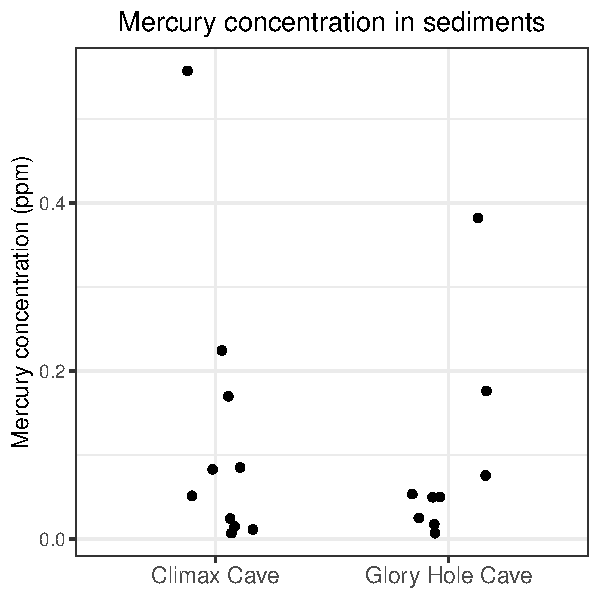
\includegraphics[height=4.0in]{dotplot_compare_sediment}
  \caption{Comparing the sediment concentrations}
  \label{fig:dotplot_compare_sediment}
\end{figure}

Because of the small sample sizes and the presence of outliers, we
cannot use the common statistical procedures, like the t-test.
Instead, we use a non-parametric test (Fisher-Pitman permutation test)
to do a hypothesis test of whether the means are significantly
different.  Not surprisingly, given the dotplot in Figure
\ref{fig:dotplot_compare_sediment}, the difference is not
significantly different (p $\approx$ 0.68).  Just to satisfy my
curiosity, I also did a non-parametric test of the variances, which
were also not significantly different.


\vspace{0.2in}


\noindent \textbf{Is it possible that bats in Climax Cave aren't
  getting past the barrel room?}

I wondered if possibly the bats in Climax Cave aren't getting further
into the cave than the barrel room and its immediate surroundings.
Let's assume they aren't, and so bat guano wouldn't have been able to
impact map locations 14-17.  Then, we exclude map locations 14-17, and
only utilize the sediments from Climax Cave map locations 2, 3, 5, and
11-13.  Figure \ref{fig:dotplot_compare_sediment_reduced} contains a
dotplot illustrating the mercury concentration in the sediments in
this reduced dataset.  Again, there is no significant difference in
mercury concentrations between the sediments in the first portion of
Climax Cave and the sediments in Glory Hole Cave (p $\approx$ 0.26).
\begin{figure}[hb]
  \centering
  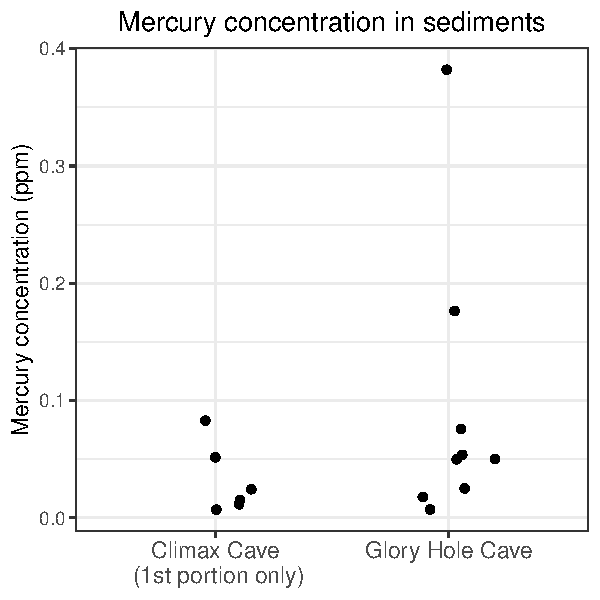
\includegraphics{dotplot_compare_sediment_reducedClimaxCave}
  \caption{Comparing the sediment concentrations between the first portion of Climax Cave and the entirety of Glory Hole Cave}
  \label{fig:dotplot_compare_sediment_reduced}
\end{figure}


\vspace{0.2in}


\noindent \textbf{Are mercury concentrations significantly different
  between sediment and guano in Climax Cave?}

Climax Cave has both guano and sediment samples, so at first I planned
to use these observations to compare whether the average mercury
levels in these two types of samples are significantly different.
Figure \ref{fig:dotplot_climaxcave_by_area} shows the mercury
concentrations in both guano and sediment samples, plotted by the cave
area from which they originated.  This figure seems to indicate the
differences in mercury concentrations are related to the portion of
the cave from which they came.  The Tee Pee Room is the only area of
the cave from which we have a mix of the two types of samples, with
one sample from guano and one from sediment.  The Barrel Room, which
was the source of the vast majority of the guano samples, has no
sediment samples for comparison.  Other than the one sample from the
Tee Pee Room, the sediment samples come from a variety of other areas
(and do not have associated guano samples).
\begin{figure}[hb]
  \centering
  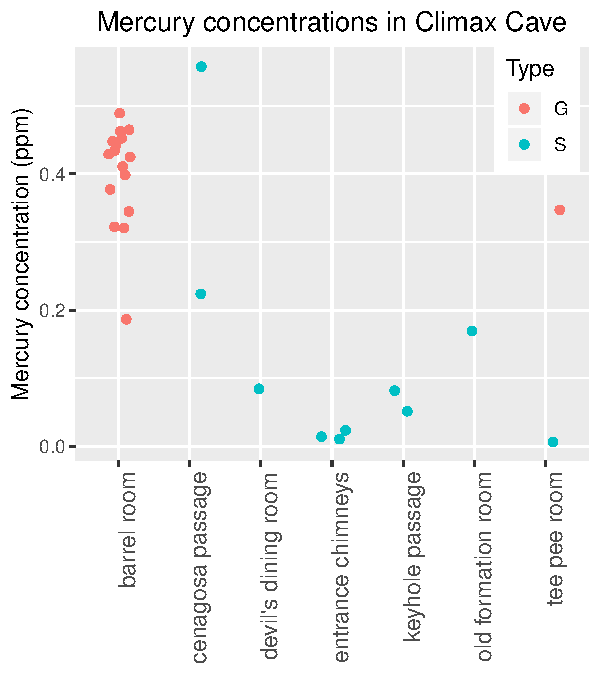
\includegraphics{dotplot_climaxcave_by_area}
  \caption{Concentrations of mercury in guano (G) and sediment (S) by area within Climax Cave}
  \label{fig:dotplot_climaxcave_by_area}
\end{figure}

This is a situation where the effect of sample type (guano
vs.\ sediment) is confounded with the effect of origin area within the
cave.  Looking at Figure \ref{fig:dotplot_climaxcave_by_area}, it
seems likely that the mercury concentrations differ by location, and
not necessarily by sample type (guano vs.\ sediment).  Because we have
a relatively small number of samples in any one room outside of the
Barrel Room, we can't use statistical techniques address the issue of
whether the mean concentrations are different among these seven areas
of Climax Cave.  However, it's noteworthy the mercury concentrations
in the sediments seem to be higher as we go deeper into the cave.  If
there are meaningful changes in the geology, animal life, etc.\ as we
go further into the cave, we might be able to group the locations in a
meaningful way.  That would allow us to consolidate the observations
into a smaller number of understandable groupings, which would
increase the sample sizes within these groups.

Nevertheless, if we do pursue the comparison between the guano and
sediments observations in Climax Cave, there is a statistically
significant difference in the mean mercury concentrations.  If we
treat the core measurements as independent, then the p-value, using
the Fisher-Pitman permutation test, is very small ($p < 0.0001$).
There could be concern about whether the core measurements are
correlated, but it's hard to tell given the small number of
observations.  If there was substantial correlation between core
samples, we would expect that the variance of these observations would
be less than that among the non-core observations.  So, I did a
non-parametric test for equality of variances, but that test result
indicated that the difference in variances is not statistically
significant.  However, if this became an issue of contention, I would
advise averaging the 10 observations taken from the guano core, even
though that reduces our effective sample size.  Even so, when we do
the Fisher-Pitman permutation test in this case, we still detect a
statistically significant difference in mean concentrations between
guano and sediments in Climax Cave, with a slightly larger p-value of
approximately 0.004.


\vspace{0.2in}


\noindent \textbf{Final questions:} I know that there are practical,
physical reasons why it's not possible to take more samples.  Also, we
cannot be expected to control where bats roost and where they don't.
However, I think we may very well receive some critiques in this vein
from future reviewers of the manuscript.  It may be a good idea to
brainstorm how we can honestly and helpfully address these kinds of
concerns, so that we can write the article with this in mind.





\end{document}
